\documentclass[a4paper,10pt,twocolumn,english]{article}

% ============================================================================
% Packages
% ============================================================================

\usepackage{babel}
\usepackage[utf8]{inputenc}
\usepackage[T1]{fontenc}
\usepackage{lmodern}
\usepackage{amsmath,amssymb,amsthm,mathtools}
\usepackage{graphicx}
\usepackage{booktabs}
\usepackage{array}
\usepackage{tabularx}
\usepackage{longtable}
\usepackage{listings}
\usepackage[table]{xcolor}
\usepackage{hyperref}
\usepackage{url}
\makeatletter
\g@addto@macro\UrlBreaks{\do\/\do\.\do\_\do\-\do\*}
\makeatother
\Urlmuskip=0mu\relax
\usepackage{enumitem}
\usepackage{microtype}
\usepackage{cleveref}
\usepackage[font=small,labelfont=bf]{caption}
\usepackage{float}
\usepackage{tikz}
\usepackage{eso-pic}
\AddToShipoutPictureBG{%
  \AtPageCenter{\makebox(0,0){\rotatebox{45}{\scalebox{8}{\textcolor[gray]{0.9}{DRAFT}}}}}%
}

% Reduce space between section number and title, prevent hyphenation in headings
\makeatletter
\renewcommand{\@seccntformat}[1]{\csname the#1\endcsname\hspace{0.5em}}
\renewcommand{\section}{\@startsection{section}{1}{\z@}%
  {-3.5ex \@plus -1ex \@minus -.2ex}%
  {2.3ex}%
  {\raggedright\normalfont\large\bfseries}}
\renewcommand{\subsection}{\@startsection{subsection}{2}{\z@}%
  {-3.25ex \@plus -1ex \@minus -.2ex}%
  {1.5ex}%
  {\raggedright\normalfont\normalsize\bfseries}}
\renewcommand{\subsubsection}{\@startsection{subsubsection}{3}{\z@}%
  {-3.25ex \@plus -1ex \@minus -.2ex}%
  {1.5ex}%
  {\raggedright\normalfont\small\bfseries}}
\makeatother
\usetikzlibrary{positioning,calc,arrows.meta}

% TikZ figure styles
\tikzset{
  figfont/.style={font=\scriptsize\sffamily},
  figbox/.style={draw, rounded corners=2pt, align=center, inner sep=4pt},
  figboxgray/.style={figbox, fill=gray!10},
  figsubbox/.style={figbox, fill=white},
  figsubboxgray/.style={figbox, fill=gray!5},
  figarrow/.style={-{Stealth[length=2mm]}, thick},
  figarrowstrong/.style={figarrow, line width=0.6pt},
}

% ============================================================================
% Typography improvements
% ============================================================================

\raggedbottom                           % Consistent local spacing
\widowpenalty=10000                     % Prevent widows (single lines at top)
\clubpenalty=10000                      % Prevent orphans (single lines at bottom)
\displaywidowpenalty=10000              % Prevent widows after display math
\predisplaypenalty=50                   % Discourage break before display math
\postdisplaypenalty=50                  % Discourage break after display math
\setlength{\emergencystretch}{2em}      % Reduce overfull lines in narrow columns
\setlength{\columnsep}{16pt}            % Slightly wider gutter for two-column reading
\setlength{\parskip}{0pt plus 1pt}      % Flexible paragraph spacing
\setlength{\floatsep}{12pt plus 3pt minus 2pt}
\setlength{\textfloatsep}{14pt plus 3pt minus 2pt}
\setlength{\intextsep}{12pt plus 3pt minus 2pt}
\setlength{\tabcolsep}{4pt}
\renewcommand{\arraystretch}{1.08}
\renewcommand{\topfraction}{0.85}       % Allow more floats at top
\renewcommand{\bottomfraction}{0.85}    % Allow more floats at bottom
\renewcommand{\textfraction}{0.10}      % Require less text on float pages
\renewcommand{\floatpagefraction}{0.7}  % Fuller float pages
\setcounter{topnumber}{2}
\setcounter{bottomnumber}{1}
\setcounter{totalnumber}{3}
\setlist[itemize]{leftmargin=*, itemsep=2pt, topsep=3pt}
\setlist[enumerate]{leftmargin=*, itemsep=2pt, topsep=3pt}
\setlist[description]{leftmargin=0pt, labelindent=0pt, itemsep=2pt, topsep=3pt}

% ============================================================================
% Numbering by section
% ============================================================================

\makeatletter
\@addtoreset{figure}{section}
\renewcommand{\thefigure}{\thesection.\arabic{figure}}
\@addtoreset{table}{section}
\renewcommand{\thetable}{\thesection.\arabic{table}}
\makeatother
\numberwithin{equation}{section}

% ============================================================================
% Theorem environments
% ============================================================================

\newtheoremstyle{paperplain}%
{6pt}{6pt}{\itshape\raggedright}{}{\bfseries}{}{0pt}%
{\thmname{#1}\thmnumber{ #2}\thmnote{. #3}.\hfill\break}
\newtheoremstyle{paperdef}%
{6pt}{6pt}{\normalfont\raggedright}{}{\bfseries}{}{0pt}%
{\thmname{#1}\thmnumber{ #2}\thmnote{. #3}.\hfill\break}
\newtheoremstyle{paperremark}%
{6pt}{6pt}{\normalfont\raggedright}{}{\itshape}{}{0pt}%
{\thmname{#1}\thmnumber{ #2}\thmnote{. #3}.\hfill\break}

\theoremstyle{paperdef}
\newtheorem{definition}{Definition}[section]

\theoremstyle{paperplain}
\newtheorem{theorem}[definition]{Theorem}
\newtheorem{lemma}[definition]{Lemma}
\newtheorem{proposition}[definition]{Proposition}
\newtheorem{corollary}[definition]{Corollary}

\theoremstyle{paperdef}
\newtheorem{example}[definition]{Example}
\newtheorem{assumption}{Assumption Block}[section]

\theoremstyle{paperremark}
\newtheorem{remark}[definition]{Remark}

% ============================================================================
% Custom commands
% ============================================================================

\newcolumntype{L}[1]{>{\raggedright\arraybackslash}p{#1}}
\newcommand{\thead}[1]{\textbf{\raisebox{0pt}[2.2ex][0.8ex]{#1}}}

\newcommand{\Coherent}{\ensuremath{\mathsf{Coherent}}}
\newcommand{\EdgeCoherent}{\ensuremath{\mathsf{EdgeCoherent}}}
\newcommand{\ActiveEdge}{\ensuremath{\mathsf{ActiveEdge}}}
\newcommand{\Consume}{\ensuremath{\mathsf{Consume}}}
\newcommand{\GEnv}{\ensuremath{\mathsf{GEnv}}}
\newcommand{\DEnv}{\ensuremath{\mathsf{DEnv}}}
\newcommand{\Hbyz}{\ensuremath{\mathsf{H}_{\mathrm{byz}}}}
\newcommand{\DeliveryModel}{\ensuremath{\mathsf{DeliveryModel}}}
\newcommand{\Obssafe}{\ensuremath{\mathsf{Obs}_{\mathrm{safe}}^{\mathrm{byz}}}}
\newcommand{\Eqsafe}{\ensuremath{\mathsf{Eq}_{\mathrm{safe}}^{\mathrm{byz}}}}
\newcommand{\Ebyz}{\ensuremath{\mathcal{E}_{\mathrm{byz}}}}
\newcommand{\ByzSafe}{\ensuremath{\mathsf{ByzSafe}}}
\newcommand{\ByzChar}{\ensuremath{\mathsf{ByzChar}}}
\newcommand{\wf}{\ensuremath{\mathsf{wf}}}
\newcommand{\consumeOne}{\ensuremath{\mathsf{consumeOne}}}
\newcommand{\RecvCompatible}{\ensuremath{\mathsf{RecvCompatible}}}
\newcommand{\EdgeShares}{\ensuremath{\mathsf{EdgeShares}}}
\newcommand{\ByzIfaceWF}{\ensuremath{\mathsf{ByzIfaceWF}}}
\newcommand{\pathref}[1]{\texttt{#1}}
\newcommand{\eqnote}[1]{\par\noindent\textit{#1.}\par\vspace{2pt}}

\newenvironment{citelist}{%
  \begin{list}{}{%
    \setlength{\leftmargin}{1.25em}%
    \setlength{\itemindent}{-1.25em}%
    \setlength{\itemsep}{2pt}%
    \setlength{\parsep}{0pt}%
    \setlength{\topsep}{3pt}}%
}{\end{list}}

\lstset{
  basicstyle=\ttfamily\footnotesize,
  keywordstyle=\color{blue},
  commentstyle=\color{gray},
  stringstyle=\color{red},
  breaklines=true,
  frame=leftline,
  rulecolor=\color{black!10},
  framerule=3pt,
  framesep=1em,
  columns=fullflexible,
  aboveskip=8pt,
  belowskip=8pt,
  xleftmargin=1.5em,
  literate={->}{$\to$\ }2 {forall}{$\forall$}1 {:=}{$\coloneqq$}2
}

% ============================================================================
% Document
% ============================================================================

\title{Coherence for Asynchronous Buffered MPST:\\A Mechanized Metatheory}
\author{Sam Hart Berman}
\date{\empty}

\begin{document}
\maketitle

\begin{abstract}
	Standard MPST uses coherence and projectability on global types to justify local safety. We define
	an operational coherence invariant $\Coherent(G,D)$ over local-type environment $G$ and buffered-trace
	environment $D$, and show that this invariant is sufficient for preservation in asynchronous semantics. The
	operational coherence invariant yields a reusable three-way edge split that avoids per-step global
	re-derivation. Lean~4 mechanization confirms our results under parameterized delivery semantics.
\end{abstract}

% ============================================================================
\section{Introduction}
\label{sec:introduction}
% ============================================================================

\subsection{Background}

Multiparty session types provide conditions under which distributed protocols execute without communication errors.
The central technical challenge is preservation: showing that each protocol step maintains
well-typedness. Binary session types use duality to ensure two-party compatibility. MPST generalizes
this property by establishing global coherence and projectability conditions.

To address preservation, the MPST field has developed projection techniques that take a global
choreography to local session types. A global type specifies the full protocol, then projection
extracts the local view for each participant. Safety means that local executions remain consistent
with their projected types.

The global--local correspondence has been a central problem since the original asynchronous
MPST formulation (Honda et al., 2008). In the global-to-local direction, projection must yield
participant behaviors that implement the global protocol. In the local-to-global direction,
one asks when participant behaviors admit a compatible global description. These directions
already have substantive solutions under specified hypotheses. In particular, Deni\'{e}lou and
Yoshida (2013) characterize a class of communicating automata and synthesize global session types
from compatible local machines. The question here concerns preserving operational compatibility
as asynchronous local states and buffered messages evolve.

Traditionally, MPST coherence and projectability conditions are formulated at the global-type level (Honda,
Yoshida, and Carbone, 2008; Honda et al., 2016; Castagna et al., 2012), with later work
refining projection criteria (Majumdar et al., 2021).

In 2008, Honda et al.\ introduced asynchronous buffered MPST. Their preservation proof was organized
around global typing and projection consistency after transitions. Many later presentations keep this
global-first organization (Honda et al., 2016; Scalas and Yoshida, 2018), while
mechanized developments continue to refine proof organization and robustness (Tirore et al., 2025).

Prior MPST literature formulates coherence at the global-type level through projectability and
well-formedness conditions. This paper refines coherence at the operational level by using
$\Coherent(G,D)$ over local environments and buffered traces. Our operational formulation makes
preservation local and compositional within the stated typed transition system, avoiding
per-step global re-derivation in these proofs. We confirm this result via Lean 4 mechanization.
Terminology note: throughout this paper, ``coherence'' denotes the operational predicate
$\Coherent(G,D)$, not the classical global-type projectability notion. Section~2 positions this
usage explicitly relative to prior MPST coherence traditions.

\subsection{Contribution}

Projection erases global structure while retaining local communication obligations.
The question is which operational invariant supports preservation after this erasure. We isolate an operational form of
coherence, $\Coherent(G,D)$, as the invariant required by our preservation proofs.
Binary session types use duality for two-party compatibility. This formulation instantiates n-ary
compatibility as receiver-buffer alignment at each active edge (Carbone et al., 2015).

$\Coherent(G,D)$ supplies the compatibility invariant for this proof architecture. Together with
typing and receiver-readiness premises, local proofs on individual edges combine to yield global
preservation. Here local-to-global reasoning means assembling edge obligations into an invariant
of the whole configuration. It does not mean synthesizing a global type from arbitrary local types.

The core contribution is one operational kernel with two theorem-level lifts: typed-step preservation
and subtype replacement. The shared kernel is edge-local checking with active-edge lifting.
For typed transitions, this kernel uses a three-way edge split.
For subtype replacement, it relies on \nolinkurl{consume_mono} under receive-compatibility.

The local-to-global shape follows standard invariant methods from program logics (Reynolds, 2002;
O'Hearn, 2007), while aligning with process-calculus decomposition tradition (Plotkin, 1981;
Milner, 1999) and Lyapunov-style invariant-function reasoning in dynamical systems (Lyapunov, 1892;
LaSalle, 1960).

\begin{figure}[H]
	\centering
	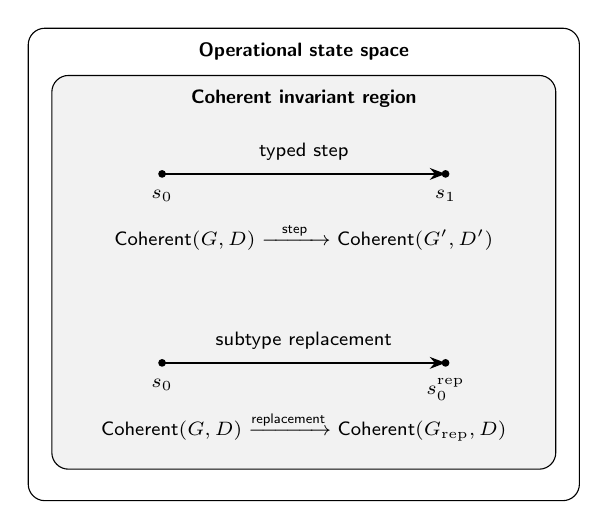
\begin{tikzpicture}[figfont, x=1mm, y=1mm]
		% State space boundary
		\draw[rounded corners=6pt] (-35,-30) rectangle (35,30);
		\node at (0,27) {\textbf{Operational state space}};

		% Coherent invariant region
		\draw[rounded corners=6pt, fill=gray!10] (-32,-26) rectangle (32,24);
		\node at (0,21) {\textbf{\textsf{Coherent} invariant region}};

		% Typed-step trajectory (top)
		\fill (-18,11.5) circle (1.4pt);
		\fill (18,11.5) circle (1.4pt);
		\draw[figarrowstrong] (-18,11.5) -- (18,11.5);
		\node[font=\scriptsize, anchor=north] at (-18,10.7) {$s_0$};
		\node[font=\scriptsize, anchor=north] at (18,10.7) {$s_1$};
		\node[anchor=south] at (0,12.0) {typed step};
		\node at (0,3.5) {$\Coherent(G,D) \xrightarrow{\text{\tiny \hphantom{en}step\hphantom{en}}} \Coherent(G',D')$};

		% Subtype-replacement trajectory (bottom)
		\fill (-18,-12.5) circle (1.4pt);
		\fill (18,-12.5) circle (1.4pt);
		\draw[figarrowstrong] (-18,-12.5) -- (18,-12.5);
		\node[font=\scriptsize, anchor=north] at (-18,-13.3) {$s_0$};
		\node[font=\scriptsize, anchor=north] at (18,-13.3) {$s_0^{\mathrm{rep}}$};
		\node[anchor=south] at (0,-12.0) {subtype replacement};
		\node at (0,-20.5) {$\Coherent(G,D) \xrightarrow{\!\text{\tiny replacement}\!} \Coherent(G_{\mathrm{rep}},D)$};
	\end{tikzpicture}
	\caption{Invariant-geometric view of preservation and subtype evolution.}
	\label{fig:p1-operational-kernel}
\end{figure}

\subsection{Scope}

This paper has two central claims. The first is Coherence preservation through a three-way split that
applies uniformly across transitions. The second is session evolution under subtype replacement via
\nolinkurl{consume_mono}, which we lift to global Coherence and progress-condition preservation under
compatibility premises.

This paper is the first in a three-part series on asynchronous buffered semantics with \DeliveryModel\ parameterization, and precisely defines the invariant kernel.
\emph{Computable Dynamics for Asynchronous MPST} develops quantitative bounds and decision procedures on that kernel.
\emph{Harmony from Coherence in Asynchronous MPST} proves reconfiguration commutation and envelope exactness.

More precisely, our contributions in this paper are as follows:
\begin{enumerate}
	\item A mechanized operational Coherence architecture with a reusable three-way edge split and typed-step wrappers that lift edge-local lemmas to preservation and progress interfaces.
	\item A message-alignment proof kernel based on \Consume, with lemmas \nolinkurl{consume_append} and \nolinkurl{consume_cons}.
	\item A subtype-replacement theorem stack from \nolinkurl{consume_mono} that preserves edge Coherence, global Coherence, and progress-side conditions under receive-compatibility premises.
	\item A premise-conditional typed effect bridge: under explicit monitor premises, handler invocations are well typed at the protocol-machine boundary, and configuration equivalence transports to observational equivalence.
\end{enumerate}

Main text proofs are proof sketches; full machine-checked derivations are provided by the Lean anchors indexed in Appendix~\ref{app:index}.
Proof-sketch template used throughout the series: state proof mode
(compositional/induction/coinduction/witness construction), give one concrete
intermediate transformation, then conclude with the claim interface.

\begin{center}
	\small
	\begin{tabularx}{\columnwidth}{@{}L{0.36\columnwidth}L{0.59\columnwidth}@{}}
		\toprule
		\thead{Symbol}  & \thead{Meaning}                                                  \\
		\midrule
		\Hbyz           & Byzantine characterization bundle                                \\
		\Obssafe        & Byzantine safety-visible observation                             \\
		\Eqsafe         & Byzantine safety-visible equality                                \\
		\Ebyz           & Byzantine determinism-envelope                                   \\
		\ByzChar        & Byzantine characterization formula                               \\
		\ByzSafe        & Byzantine safety predicate                                       \\
		\ByzIfaceWF     & Byzantine interface well-formedness                              \\
		\Coherent       & global active-edge compatibility                                 \\
		\EdgeCoherent   & edge-local compatibility check                                   \\
		\EdgeShares     & edge-to-endpoint incidence predicate                             \\
		\Consume        & trace-to-type alignment function                                 \\
		\GEnv           & endpoint-to-local-type environment                               \\
		\DEnv           & edge-to-buffered-trace environment                               \\
		$(G,D)$         & configuration pair of local-type and buffered-trace environments \\
		$s_i$           & illustrative configuration states in traces/figures              \\
		$q$             & quotient projection to symmetry classes                          \\
		$\sim$          & coherence-preserving symmetry/equivalence relation               \\
		\ActiveEdge     & endpoint-presence guard                                          \\
		\RecvCompatible & receive-side replacement compatibility                           \\
		\DeliveryModel  & parametric delivery interface                                    \\
		$N_s$           & explored state count in finite checker objects                   \\
		$N_e$           & explored transition-edge count in finite checker objects         \\
		$L_{\max}$      & maximum active-edge buffered trace length                        \\
		$W_{\max}$      & maximum size of checked witness/certificate object               \\
		\bottomrule
	\end{tabularx}
	\captionof{table}{Notation used in this paper.}
\end{center}

% ============================================================================
\section{Model and Semantics}
\label{sec:model}
% ============================================================================

Configurations are represented by endpoint and edge environments. \GEnv{} maps endpoints to local types, \DEnv{} maps directed edges to buffered type traces, and \texttt{Buffers} maps directed edges to runtime payload queues.

\begin{table}[H]
	\centering
	\small
	\begin{tabularx}{\columnwidth}{@{}L{0.55\columnwidth}L{0.4\columnwidth}@{}}
		\toprule
		\thead{Assumption}              & \thead{Status}       \\
		\midrule
		asynchronous buffered semantics & required             \\
		active-edge quantification      & required             \\
		fair scheduling profile         & assumed where stated \\
		\DeliveryModel param.           & required             \\
		crash-stop and Byzantine claims & interface claim only \\
		\bottomrule
	\end{tabularx}
	\caption{Model assumptions for exact statements in this paper.}
\end{table}

\begin{assumption}[Core Model Premises]
	\label{assump:p1-core}
	Core claims in this paper assume asynchronous buffered semantics, active-edge quantification, and \DeliveryModel parameterization. Fair scheduling assumptions apply where stated.
\end{assumption}

Assumption-block inheritance policy. Assumption blocks do not inherit implicitly. If a theorem does not name a block, it uses Assumption Block~\ref{assump:p1-core} only.

\begin{definition}[Active Edge]
	$\ActiveEdge(G, e)$ holds when both endpoints of edge $e$ are present in $G$.
\end{definition}

\begin{definition}[Edge Coherence]
	$\EdgeCoherent(G, D, e)$ holds when the receiver side can consume the buffered trace on edge $e$ under the local type in $G$.
\end{definition}

\begin{definition}[Coherence]
	$\Coherent(G, D)$ holds when every active edge is edge coherent.
\end{definition}

\begin{definition}[Well-Typed Configuration and Step]
	Write $\Gamma \vdash (G,D)\ \wf$ for configuration typing and
	$\Gamma \vdash (G,D)\to(G',D')$ for one-step typing in the operational
	fragment used by this paper.
\end{definition}

Role split. Well-typedness constrains rule formation and environment-domain
consistency. Coherence constrains edge-local message and type compatibility.

\begin{definition}[consumeOne]
	For source role $r$, value type $T$, and local type $L$:
	write $\consumeOne_{r,T}(L):=\consumeOne(r,T,L)$. Then
	\[
		\begin{aligned}[t]
			\consumeOne_{r,T}(\mathsf{recv}(r,T,L')) & = \mathsf{some}(L'),                  \\
			\consumeOne_{r,T}(L)                     & = \mathsf{none}\quad\text{otherwise.}
		\end{aligned}
	\]
	Here $\mathsf{NonRecvHeads}$ abbreviates
	$\{\mathsf{send},\mathsf{select},\mathsf{branch},\mathsf{end},\mathsf{var}\}$.
	``Otherwise'' means $L\in\mathsf{NonRecvHeads}$ or $L=\mu L_0$ at this layer.
	Head checks are therefore constructor-local. Recursive unfolding is handled by
	the local-type normalization layer before this head check.
\end{definition}

\begin{definition}[Consume]
	For source role $r$, receiver local type $L$, and buffered trace $ts$:
	\noindent\begin{minipage}{\columnwidth}
		\begin{lstlisting}
Consume r L [] := some L
Consume r L (T :: ts) :=
  match consumeOne r T L with
  | some L' => Consume r L' ts
  | none    => none
\end{lstlisting}
	\end{minipage}
	The recursion is structural on trace length.
\end{definition}

\begin{definition}[Guarded Recursion Premise]
	A recursive local type satisfies $\mathsf{GuardedMu}$ when every bound-variable
	occurrence in a $\mu$-body appears under a communication constructor. This
	excludes unguarded heads that can unfold forever without consuming input.
\end{definition}

Termination measure. Define
\begin{equation}
	\label{eq:p1-consume-measure}
	\mu_{\Consume}(L,ts) := |ts|.
\end{equation}
If a recursive call is taken, the argument changes from $(L,T::ts)$ to
$(L',ts)$, so $\mu_{\Consume}$ strictly decreases by one. Hence recursion is
well-founded on natural numbers.

Recursive local types. For $\mu$-types, unfolding is handled in the
normalization layer and does not add recursive depth to $\Consume$ itself,
because $\Consume$ recursion is indexed only by trace length. Under
$\mathsf{GuardedMu}$, normalization cannot generate infinite head-unfolding
chains in the well-typed fragment used here.

Mechanized anchors for this block are
\nolinkurl{consume_one_depth_lt},
\nolinkurl{consume_length_le_depth},
\nolinkurl{LocalTypeR.guarded_full_unfold_not_var}, and
\nolinkurl{mu_height_substitute_guarded}.

\begin{definition}[Byzantine Interface Well-Formedness]
	$\ByzIfaceWF(G, D)$ is the interface predicate used for Byzantine-facing statements in this paper. It is defined on paper as an alias of $\Coherent(G, D)$; the current Lean artifact has no separate anchor for it.
\end{definition}

Delivery behavior is parameterized by \DeliveryModel. This gives one theorem shape across FIFO, causal, and lossy instances. The interface laws and instance examples appear in Appendix~\ref{app:delivery}.
\begin{equation}
	\label{eq:p1-active-edge-boundary}
	\begin{aligned}[t]
		\Coherent(G,D)\ :=\ \forall e,\ \ActiveEdge(G,e)
		\\
		\to\ \EdgeCoherent(G,D,e).
	\end{aligned}
\end{equation}
Edges incident to absent endpoints are excluded by $\ActiveEdge$.

\subsection{Operational Coherence}

In this paper, ``coherence'' means the operational invariant
$\Coherent(G,D)$ from Equation~\ref{eq:p1-active-edge-boundary}: every active edge must satisfy
$\EdgeCoherent$.

This is aligned with, but distinct from, classical MPST coherence/projectability on global types
(Honda et al., 2008; Honda et al., 2016; Castagna et al., 2012; Majumdar et al., 2021) and logical
n-ary coherence accounts (Carbone et al., 2015; Carbone et al., 2016; Carbone et al., 2017).
The present claim is operational and proof-architectural, not a denotational identification of models.

The compatibility intuition follows coherence-space/session-logic lineages (Girard, 1987; Caires and
Pfenning, 2010; Wadler, 2012) and the communicating-automata compatibility tradition
(Gay and Hole, 2005; Deni\'{e}lou and Yoshida, 2012; Brand and Zafiropulo, 1983): local compatibility
obligations aggregate into one global invariant used by preservation.

\begin{table}[H]
	\centering
	\footnotesize
	\begin{tabularx}{\columnwidth}{@{}L{0.34\columnwidth}L{0.54\columnwidth}@{}}
		\toprule
		\thead{Coherence-space}       & \thead{Operational in This Paper}                             \\
		\midrule
		token                         & active-edge obligation for directed edge $e$                  \\
		coherence relation            & $\EdgeCoherent(G,D,e)$                                        \\
		clique                        & $\Coherent(G,D)$ over all active edges                        \\
		preservation of compatibility & one-step preservation (Thm.~\ref{thm:coherence-preservation}) \\
		\bottomrule
	\end{tabularx}
	\caption{Compatibility correspondence used as operational intuition (not a formal embedding claim).}
\end{table}

% ============================================================================
\section{Worked Example}
\label{sec:example}
% ============================================================================

We illustrate coherence preservation through a three-role protocol that exercises the key proof obligations. These include active-edge checks, buffer compatibility via \Consume, and the three-way edge split for typed steps. The configuration includes a non-empty buffer to demonstrate how in-flight messages interact with local-type advancement.

\noindent\begingroup\raggedright
\textbf{Running example.} Roles are \texttt{C} (client), \texttt{P} (pool), and \texttt{M} (monitor), with global interaction:
\par\endgroup

\noindent\begin{minipage}{\columnwidth}
	\begin{lstlisting}
C -> P : Request(n)
P -> C : Grant(k)
C -> M : Report(k)
M -> P : Confirm
P -> C : Token(t)
\end{lstlisting}
\end{minipage}

Fix local continuations:

\noindent\begin{minipage}{\columnwidth}
	\begin{lstlisting}
L_C := recv P Grant(k);
       send M Report(k);
       recv P Token(t); end
L_P := recv M Confirm;
       send C Token(t); end
L_M := recv C Report(k);
       send P Confirm; end
\end{lstlisting}
\end{minipage}

and in-flight configuration $(G_0,D_0)$:

\noindent\begin{minipage}{\columnwidth}
	\begin{lstlisting}
G_0(C) = L_C
G_0(P) = L_P
G_0(M) = L_M
D_0(P,C) = [Grant(k)]
D_0(e)   = []    for e != (P,C)
\end{lstlisting}
\end{minipage}

Assume typing judgment $\Gamma \vdash (G_0,D_0)\ \wf$.

The active-edge obligation is:
\begin{equation}
	\forall e,\ \ActiveEdge(G_0,e)\to \EdgeCoherent(G_0,D_0,e).
\end{equation}
The example is used via the following derived rule instances.

	{\footnotesize
		\begin{gather}
			\dfrac{
				\Gamma \vdash (G_0,D_0)\ \wf \quad D_0(P,C){=}[\mathrm{Grant}(k)]
			}{
				(G_0,D_0){\to}(G_1,D_1) \land \Coherent(G_1,D_1)
			}\hspace{0.75em}
			\\[10pt]
			\dfrac{
				\Gamma \vdash (G_1,D_1)\ \wf \quad \text{\texttt{consume\_append}}
			}{
				(G_1,D_1){\to}(G_2,D_2) \land \Coherent(G_2,D_2)
			}\hspace{0.75em}
			\\[10pt]
			\dfrac{
				\Coherent(G_0,D_0) \quad \RecvCompatible(G_0,G'_0)
			}{
				\Coherent(G'_0,D_0)
			}\hspace{0.75em}
		\end{gather}
		\vspace{6pt}
	}

For the step edge $u=(C,M)$ with stepped endpoint $ep_{\mathrm{step}}$, the case split used later is: updated ($e=u$), shared-endpoint ($e\neq u \land \EdgeShares(e,ep_{\mathrm{step}})$), and unrelated ($e\neq u \land \neg\EdgeShares(e,ep_{\mathrm{step}})$).

% ============================================================================
\section{Coherence Preservation Architecture}
\label{sec:preservation}
% ============================================================================

Running-example thread. Section~\ref{sec:example} instantiates this theorem on
the baseline C/P/M trace and its one-step send-recv transitions.

\begin{figure}[H]
	\centering
	\resizebox{\columnwidth}{!}{%
		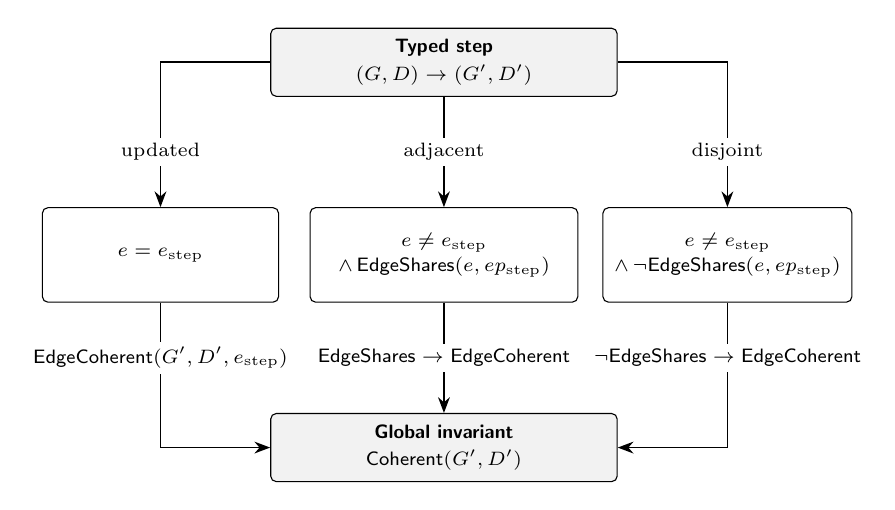
\begin{tikzpicture}[figfont]
			% Typed step at top
			\node[figboxgray, minimum width=44mm] (step)
			{\textbf{Typed step}\\[2pt] $(G,D)\to(G',D')$};

			% Three-way split: predicate boxes only (case names on arrows)
			\node[figsubbox, below=14mm of step, xshift=-36mm, minimum width=30mm, minimum height=12mm] (updated)
			{$e=e_{\mathrm{step}}$};
			\node[figsubbox, below=14mm of step, minimum width=34mm, minimum height=12mm] (shared)
			{$e\neq e_{\mathrm{step}}$\\[1pt] $\land\,\EdgeShares(e,ep_{\mathrm{step}})$};
			\node[figsubbox, below=14mm of step, xshift=36mm, minimum width=30mm, minimum height=12mm] (unrel)
			{$e\neq e_{\mathrm{step}}$\\[1pt] $\land\,\neg\EdgeShares(e,ep_{\mathrm{step}})$};

			\node[figboxgray, below=14mm of shared, minimum width=44mm] (global)
			{\textbf{Global invariant}\\[2pt] $\Coherent(G',D')$};

			% Labeled arrows from step to each case
			\draw[figarrowstrong] (step) -- (shared);
			\draw[figarrowstrong] (step.west) -- (updated.north |- step.west) -- (updated.north);
			\draw[figarrowstrong] (step.east) -- (unrel.north |- step.east) -- (unrel.north);
			\coordinate (label-y-top) at ($(step.south)!0.5!(shared.north)$);
			\node[font=\scriptsize, fill=white, inner sep=2pt] at (updated |- label-y-top) {updated};
			\node[font=\scriptsize, fill=white, inner sep=2pt] at (shared |- label-y-top) {adjacent};
			\node[font=\scriptsize, fill=white, inner sep=2pt] at (unrel |- label-y-top) {disjoint};

			% Labeled arrows from cases to global invariant
			\draw[figarrowstrong] (updated.south) |- (global.west);
			\draw[figarrowstrong] (shared.south) -- (global.north);
			\draw[figarrowstrong] (unrel.south) |- (global.east);
			\coordinate (label-y-bot) at ($(shared.south)!0.5!(global.north)$);
			\node[font=\scriptsize, fill=white, inner sep=2pt] at (updated |- label-y-bot) {$\EdgeCoherent(G',D',e_{\mathrm{step}})$};
			\node[font=\scriptsize, fill=white, inner sep=2pt] at (shared |- label-y-bot) {$\EdgeShares \to \EdgeCoherent$};
			\node[font=\scriptsize, fill=white, inner sep=2pt] at (unrel |- label-y-bot) {$\neg\EdgeShares \to \EdgeCoherent$};
		\end{tikzpicture}
	}%
	\caption{Three-way edge split used by the preservation proof. Top node is the
		typed step $(G,D)\to(G',D')$. Middle nodes are the exhaustive edge classes
		(updated, adjacent/shared-endpoint, disjoint). Bottom node is the global
		post-step invariant. Arrow labels state the obligation discharged per class.}
	\label{fig:p1-preservation-architecture}
\end{figure}

\begin{theorem}[Coherence Preservation]
	\label{thm:coherence-preservation}
	Under Assumption Block~\ref{assump:p1-core}, for all environments $G,D,G',D'$, if $(G,D) \to (G',D')$ is a well-typed step in the send and recv and select and branch fragment, then
	\begin{equation}
		\Coherent(G,D) \implies \Coherent(G',D').
	\end{equation}
	This claim is exact for one-step preservation in the stated core rule fragment.
\end{theorem}

Premise roles. In Theorem~\ref{thm:coherence-preservation}, well-typedness
selects the applicable operational rule and preserves structural side
conditions, while Coherence provides the edge obligations transported by the
three-way split.

Running-example instantiation. In Section~\ref{sec:example}, each checked
transition in the baseline protocol is one of the send/recv/select/branch
steps covered by this theorem.

\begin{lemma}[Three-Way Edge-Split Exhaustiveness]
	\label{lem:p1-edge-split-exhaustive}
	Fix stepped edge $u$ and stepped endpoint $ep_{\mathrm{step}}$. For any edge $e$,
	exactly one of the following holds:
	\[
		\begin{aligned}[t]
			e & =u,                                                \\
			e & \neq u\land \EdgeShares(e,ep_{\mathrm{step}}),     \\
			e & \neq u\land \neg\EdgeShares(e,ep_{\mathrm{step}}).
		\end{aligned}
	\]
\end{lemma}

\begin{proof}[Proof sketch]
	Case-split first on $e=u$. If false, split on the Boolean incidence predicate
	$\EdgeShares(e,ep_{\mathrm{step}})$. This yields the two remaining cases and
	excludes overlap by propositional contradiction. Graph-theoretically, this is
	the partition of all non-updated edges into those incident to the stepped
	endpoint and those not incident to it. The mechanized splitter is
	\nolinkurl{edge_case_split}.
\end{proof}

\begin{proof}
	Fix a well-typed one-step transition
	\[
		(G,D)\to(G',D')
	\]
	in the send/recv/select/branch fragment, and assume $\Coherent(G,D)$.
	To prove $\Coherent(G',D')$, let $e$ be arbitrary and assume $\ActiveEdge(G',e)$.
	It suffices to show $\EdgeCoherent(G',D',e)$.

	Apply \nolinkurl{edge_case_split} to $e$ with respect to the stepped edge $e_{\mathrm{step}}$
	and stepped endpoint $ep_{\mathrm{step}}$. Exactly one of the following holds:
	\[
		\begin{aligned}[t]
			e & = e_{\mathrm{step}},                                               \\
			e & \neq e_{\mathrm{step}}\land \EdgeShares(e,ep_{\mathrm{step}}),     \\
			e & \neq e_{\mathrm{step}}\land \neg\EdgeShares(e,ep_{\mathrm{step}}).
		\end{aligned}
	\]

	\textbf{Case 1 (updated edge).}
	Here $e=e_{\mathrm{step}}$.
	The post-step edge obligation is discharged by the rule-local preservation theorem corresponding
	to the operational rule used by $(G,D)\to(G',D')$:
	send/recv/select/branch map to
	\nolinkurl{coherent_send_preserved},
	\nolinkurl{coherent_recv_preserved},
	\nolinkurl{coherent_select_preserved},
	\nolinkurl{coherent_branch_preserved}.
	The message/type-alignment subgoal is reduced to $\Consume$ lemmas:
	send/select use \nolinkurl{consume_append} for enqueue extension, recv/branch use
	\nolinkurl{consume_cons} for aligned head-consumption and continuation alignment.
	Hence $\EdgeCoherent(G',D',e)$.
	In the running example (Section~\ref{sec:example}), this is the direct case
	for the currently stepped channel edge.

	\textbf{Case 2 (shared endpoint, not updated edge).}
	Assume
	$e\neq e_{\mathrm{step}}\land \EdgeShares(e,ep_{\mathrm{step}})$.
	From pre-state coherence and active-edge premises on unchanged incident structure, we have
	$\EdgeCoherent(G,D,e)$. The shared-endpoint transport lemmas preserve receiver projection and the
	relevant buffered segment on $e$, so the same consumption witness transports to the post-state.
	Therefore $\EdgeCoherent(G',D',e)$.

	\textbf{Case 3 (unrelated edge).}
	Assume
	$e\neq e_{\mathrm{step}}\land \neg\EdgeShares(e,ep_{\mathrm{step}})$.
	No endpoint or buffer component of $e$ is touched by the step; frame transport gives
	invariance of edge-local coherence on $e$ between $(G,D)$ and $(G',D')$. Since
	$\Coherent(G,D)$, we obtain $\EdgeCoherent(G',D',e)$.

	All cases yield $\EdgeCoherent(G',D',e)$ for arbitrary active $e$, hence
	\[
		\forall e,\ \ActiveEdge(G',e)\to \EdgeCoherent(G',D',e),
	\]
	which is $\Coherent(G',D')$.
\end{proof}

The split operator is implemented by \nolinkurl{edge_case_split}. Rule-level preservation lemmas are grouped by send, recv, select, and branch cases. Table~\ref{tab:p1-index} gives the anchor-to-file mapping, and \cref{app:chains} records theorem-to-lemma chains.

The architecture is quotient-first. The concrete step relation induces dynamics on equivalence classes once coherence-preserving symmetries are quotiented out.

The quotienting step should be read as symmetry reduction. Distinct interleavings that are equivalent under the symmetry relation are identified as one observable class. Formally, the induced square is:
\begin{definition}[Observational Quotient Relation]
	For coherent configurations $X,Y$, write $X\sim Y$ iff their runtime
	realizations are equivalent under the configuration-equivalence/effect-bisimulation
	bridge used in this paper (equivalently, effect-bisimilar modulo silent steps
	at the observational interface).
\end{definition}
\noindent
Relation note. This paper writes the quotient as $\sim$; the same bridge-level
relation is named \texttt{ConfigEquiv} in Paper 3. The quotient collapses silent
internal monitor steps and symmetry-equivalent reorderings that preserve
safety-visible observations.
Canonical alias across the series: on coherent configurations, $(G_1,D_1)\sim
	(G_2,D_2)$ iff \texttt{ConfigEquiv}$((G_1,D_1),(G_2,D_2))$ at the observational
boundary defined in Paper 3 (Configuration Equivalence definition). Scope is
the same in both papers: coherent/admitted states only.

\noindent
\vspace{-2pt}
\begin{equation}
	\label{eq:p1-quotient-commute}
	q(\mathsf{step}(G,D))\ =\ \mathsf{step}_{/ \sim}(q(G,D)).
\end{equation}
Here $q$ is the quotient projection map and $\sim$ is the coherence-preserving equivalence relation used by the bridge layer.
Equation~\ref{eq:p1-quotient-commute} states the commuting condition used across these three papers.

\begin{lemma}[Step Congruence Under $\sim$]
	\label{lem:p1-quotient-congruence}
	For coherent pre-states $(G_1,D_1)$ and $(G_2,D_2)$, if
	\[
		(G_1,D_1)\sim(G_2,D_2)
	\]
	and
	\[
		(G_1,D_1)\to(G_1',D_1'),
	\]
	then there exists $(G_2',D_2')$ such that
	\[
		(G_2,D_2)\to(G_2',D_2')
	\]
	and
	\[
		(G_1',D_1')\sim(G_2',D_2').
	\]
\end{lemma}

\begin{proof}[Proof sketch]
	Use the configuration-equivalence and effect-bisimulation bridge
	(\nolinkurl{config_equiv_iff_effect_bisim_silent} and
	\nolinkurl{effect_bisim_implies_observational_equivalence}) to transport one
	step across $\sim$-equivalent pre-states. Then apply
	Theorem~\ref{thm:coherence-preservation} to keep post-states in the coherent
	domain of the quotient relation.
	This argument is compositional at the one-step level: first transport the
	operational step across the quotient, then compose with preservation on the
	target side. No separate induction is needed because the statement is single-step.
\end{proof}

The commuting equation above is therefore read as preservation plus
Lemma~\ref{lem:p1-quotient-congruence}, which makes $\mathsf{step}_{/\sim}$
well-defined on quotient classes.

The case partition used by \nolinkurl{edge_case_split} is:
\eqnote{Case partition for checked edge}
Here $S(e):=\EdgeShares(e,ep_{\mathrm{step}})$.
\begin{equation}
	\begin{aligned}
		\mathsf{updated}   & :\ e=u;                    \\
		\mathsf{shared}    & :\ e\neq u\land S(e);      \\
		\mathsf{unrelated} & :\ e\neq u\land \neg S(e).
	\end{aligned}
\end{equation}
The three branches are discharged by updated-edge preservation, shared-endpoint transport, and unrelated-edge frame transport, respectively.

% ============================================================================
\section{Message-Type Alignment via Consume}
\label{sec:consume}
% ============================================================================

$\Consume$ is the proof kernel for message-type alignment. It removes most rule-specific structural complexity from preservation proofs.

\begin{lemma}[consume\_append]
	Consumption over concatenated traces factors through sequential consumption.
\end{lemma}

\begin{lemma}[consume\_cons]
	Head consumption reduces to one-step alignment plus recursive continuation alignment.
\end{lemma}

\begin{proof}[Proof sketch]
	The library is centered on $\consumeOne$ and structural recursion on trace shape.

	\begin{enumerate}
		\item \nolinkurl{consume_append}: induction on trace prefix $ts$; base case $ts = []$ is immediate by simplification ($L' = L_r$); step case peels one $\consumeOne$ transition and applies induction hypothesis to the residual local type.
		\item \nolinkurl{consume_cons}: unfold one $\Consume$ step on head $T$; case split on $\consumeOne(\mathit{from}, T, L_r)$; resulting equation is definitional in both branches.
		\item Preservation integration: send/select proofs use \nolinkurl{consume_append} to justify extending buffered traces; recv/branch proofs use \nolinkurl{consume_cons} to justify consuming the head message and continuing.
	\end{enumerate}

	This isolates alignment complexity into two reusable lemmas rather than duplicating ad-hoc trace reasoning in each operational rule.
\end{proof}

For the worked example, \nolinkurl{consume_cons} discharges the \texttt{Grant} receive step at \texttt{C} by reducing the obligation to continuation coherence after one aligned message.

Complexity note (checker vs runtime). Under constant-time constructor tests in
\consumeOne, one \Consume check on edge trace $ts_e$ costs $O(|ts_e|)$.
Therefore one full active-edge Coherence \emph{checker} pass costs
\[
	O\!\Big(\sum_{e\in E_{\mathrm{active}}}|ts_e|\Big)=O(N_e\cdot L_{\max}),
\]
where $N_e:=|E_{\mathrm{active}}|$ and
$L_{\max}:=\max_{e\in E_{\mathrm{active}}}|ts_e|$. Runtime \emph{system-step}
cost is separate: this bound is for validation/checking, not for the
operational transition relation itself.

% ============================================================================
\section{Session Evolution via Subtyping}
\label{sec:evolution}
% ============================================================================

Running-example thread. Section~\ref{sec:example} gives the concrete endpoint
state that is refined by this replacement theorem.

Session evolution replaces one endpoint local type with a compatible refinement and asks whether coherence is preserved.

This replacement argument follows a standard commutation intuition from trace-equivalence and commuting-conversion lines. The standard point is that local reorderings or local refinements should preserve observable behavior when compatibility conditions hold. What is new here is an operational criterion for asynchronous subtype replacement that is stated directly through \nolinkurl{consume_mono} and discharged with edge-local coherence obligations.

\begin{assumption}[Replacement Compatibility]
	\label{assump:p1-replacement}
	The subtype-evolution theorem assumes $G(ep)=\mathsf{some}(L_1)$, $G_{\mathrm{rep}} = G[ep\mapsto L_2]$ (so the typing domain is preserved and all other endpoints are unchanged), and $\RecvCompatible(r,L_1,L_2)$ for every sender role $r$ (every trace $L_1$ can consume, $L_2$ can also consume).
\end{assumption}

\begin{theorem}[Session Evolution via \nolinkurl{consume_mono}]
	\label{thm:session-evolution}
	For all endpoints $ep$ and environments $G,D,G_{\mathrm{rep}}$, if Assumption Block~\ref{assump:p1-replacement} holds for replacement at $ep$, then
	\begin{equation}
		\Coherent(G,D) \implies \Coherent(G_{\mathrm{rep}},D).
	\end{equation}
	This claim is exact for type replacement steps covered by Assumption Block~\ref{assump:p1-replacement}.
\end{theorem}

Running-example instantiation. In Section~\ref{sec:example}, replacing one
receiver continuation by a compatible subtype is an instance of this theorem.

\begin{proof}[Proof sketch]
	The replacement theorem is proved by a monotonicity-to-global-lift chain.

	\begin{enumerate}
		\item Local monotonicity: establish receive-compatibility ($\RecvCompatible$) between old and replacement local types; apply \nolinkurl{consume_mono} to show every successful old consumption remains successful after replacement.
		\item Edge lift: use \nolinkurl{edge_coherent_type_replacement} on edges targeting the replaced endpoint; for non-target edges, transport coherence by environment agreement.
		\item Global lift: combine edge cases to derive \nolinkurl{coherent_type_replacement}.
		\item Progress compatibility: \nolinkurl{progress_conditions_type_replacement} preserves the progress-side conditions $\mathsf{HeadCoherent}$, $\mathsf{RoleComplete}$, and $\mathsf{ValidLabels}$ under the same replacement.
	\end{enumerate}
	In the running example, this appears as refining the continuation after the
	first request/grant exchange while preserving all edge checks.

	Hence compatible subtype replacement preserves Coherence without re-running global derivations.
\end{proof}

Core lemmas are in the subtype-replacement core and liveness layers.
The subtype-replacement commutation principle and proof-lift chain are:
\begin{equation}
	\begin{aligned}[t]
		\Coherent(G,D)\ \land\ \mathsf{Compat}_{ep}(G,G_{\mathrm{rep}})
		\\
		\Longrightarrow\ \Coherent(G_{\mathrm{rep}},D).
	\end{aligned}
\end{equation}
\begin{equation}
	\texttt{consume\_mono}\ \Longrightarrow\ \text{edge lift}\ \Longrightarrow\ \text{global lift}.
\end{equation}
with compatibility discharged by \nolinkurl{consume_mono} and replacement side conditions.

% ============================================================================
\section{Effect-Typed Bridge}
\label{sec:bridge}
% ============================================================================

\texttt{EffectSpec.handlerType} records typed effect obligations at the VM (protocol-machine) boundary.
The session-facing instruction forms used in this paper are \texttt{send}, \texttt{receive}, \texttt{offer},
\texttt{choose}, and \texttt{invoke} (the Lean \texttt{WellTypedInstr} relation also covers guard
\texttt{acquire}/\texttt{release} and session \texttt{open}). \texttt{WellTypedInstr} relates each
instruction to a pre- and post-local type: \texttt{send} and \texttt{receive} advance a send/recv
type to its continuation, \texttt{offer} advances a select type along a listed branch, \texttt{choose}
requires every jump-table label to be covered by a branch, and \texttt{invoke} types a handler step from
\texttt{EffectSpec.handlerType} to \texttt{end}. \Consume-alignment is not part of \texttt{WellTypedInstr};
it is carried by the Coherence layer of Sections~\ref{sec:preservation}--\ref{sec:evolution}.
Write this mapping as
\begin{equation}
	\begin{aligned}[t]
		\mathsf{WTObl}(\texttt{send})   & = \mathsf{SendCont},         \\
		\mathsf{WTObl}(\texttt{receive}) & = \mathsf{RecvCont},         \\
		\mathsf{WTObl}(\texttt{offer})   & = \mathsf{SelectBranchCont}, \\
		\mathsf{WTObl}(\texttt{choose})  & = \mathsf{BranchCover},      \\
		\mathsf{WTObl}(\texttt{invoke}) & = \mathsf{InvokeLift}.
	\end{aligned}
\end{equation}
where each right-hand side names the corresponding constructor family of \texttt{WellTypedInstr}.

Effect-bisimulation primer. Two configurations are effect-bisimilar when they
match on the same observable effect trace up to silent internal steps. In this
paper, effect-bisimulation is the bridge quotient because bridge soundness is
an observational claim, and silent monitor-internal variation should not change
that claim.

\begin{table}[H]
	\centering
	\scriptsize
	\begin{tabularx}{\columnwidth}{@{}L{0.28\columnwidth}L{0.62\columnwidth}@{}}
		\toprule
		\thead{Instruction Form}         & \thead{Session-Side Typing Obligation}              \\
		\midrule
		\texttt{send}                    & send type advances to its continuation              \\
		\texttt{receive}                 & recv type advances to its continuation              \\
		\texttt{offer}                   & select type advances along a listed branch          \\
		\texttt{choose}                  & jump-table labels covered by branch labels          \\
		\texttt{invoke}                  & \texttt{EffectSpec.handlerType} to \texttt{end}     \\
		\bottomrule
	\end{tabularx}
	\caption{VM instruction-layer summary used by the bridge theorem.}
\end{table}

\begin{proposition}[Bridge Soundness]
	\label{prop:bridge-soundness}
	Under Assumption Block~\ref{assump:p1-core}, let $m$ be a session monitor satisfying the predicates \nolinkurl{monitor_sound} and \nolinkurl{unified_monitor_preserves} (these are premises, not proved properties of a particular monitor). Then for any handler $h$ and effect action $a$: (i) \texttt{invoke}~$a$ on $h$ is well typed from \texttt{EffectSpec.handlerType}~$a$ to \texttt{end}, as is every action of any handler fragment or declared effect interface; (ii) if $m$ steps from handler $h$ then the session identifier is preserved; and (iii) for any configurations $C_1,C_2$ with $\texttt{ConfigEquiv}(C_1,C_2)$, $C_1$ and $C_2$ are observationally equivalent under the configuration-erasure observation.
\end{proposition}

\begin{proof}[Proof sketch]
	The bridge composition has three steps.
	\begin{enumerate}
		\item Build \texttt{ProtocolMachineBridgePremises} from \nolinkurl{monitor_sound}, \nolinkurl{unified_monitor_preserves}, and the \nolinkurl{WellTypedInstr.wt_invoke} constructor (\nolinkurl{protocol_machine_bridge_premises_of_monitor}).
		\item Lift handler typing to fragments and monitor steps through \nolinkurl{handler_obligation_local}, \nolinkurl{handler_fragment_typing_of_premises}, and \nolinkurl{handler_protocol_machine_step_typing}.
		\item Compose with observational transport via \nolinkurl{protocol_machine_bridge_soundness_composed}, which uses \nolinkurl{config_equiv_iff_effect_bisim_silent} and \nolinkurl{effect_bisim_implies_observational_equivalence}.
	\end{enumerate}
	Equivalently, with $\mathsf{BridgePrem}(h)$ abbreviating the listed premises,
	\[
		\begin{aligned}[t]
			\mathsf{BridgePrem}(h)
			 & \Longrightarrow \mathsf{InstrTyped}(h) \\
			 & \land \mathsf{ObsTransport}(h).
		\end{aligned}
	\]
	Therefore runtime typing obligations and observational transport both hold under the stated premises.
\end{proof}

\begin{assumption}[Byzantine Interface Premises]
	\label{assump:p1-byzantine}
	The interface statements in this section assume shared notation for \Hbyz, \Obssafe, \Eqsafe, and \Ebyz, plus theorem-pack capability naming consistency between abstract and runtime layers.
\end{assumption}

\begin{remark}[Byzantine Interface Convention (BZ-1)]
	\label{thm:bz1}
	Under Assumption Block~\ref{assump:p1-byzantine}, Byzantine safety-track statements in this series are interpreted on configurations $(G,D)$ satisfying $\ByzIfaceWF(G,D)$, i.e.\ $\Coherent(G,D)$. Unfolding the definition, every active edge carries the same sender-existence and $\Consume$ obligations as the Coherence layer. This is a definitional convention, not a separate theorem; the current Lean artifact does not mechanize a dedicated Byzantine interface layer.
\end{remark}

\begin{remark}[Dropped-Assumption Witnesses (BZ-1.1)]
	\label{cor:bz1-1}
	Under Assumption Block~\ref{assump:p1-byzantine}, if a later construction provides a witness violating \ByzSafe when an assumption class named in \Hbyz{} is dropped, we intend that witness to be stated against the same active-edge Coherence interface. This is a scoping convention for later papers, not a mechanized result.
\end{remark}

\begin{remark}[Capability-Gated VM Interface (BZ-1.2)]
	\label{prop:bz1-2}
	The Lean theorem pack defines a Boolean runtime gate \texttt{canOperateUnderByzantineEnvelope} that holds exactly when a theorem pack carries both a Byzantine-safety profile and protocol-machine envelope-adherence evidence; operation under the Byzantine envelope is refused otherwise. The gate checks the presence of evidence only. Interpretation of safety-visible obligations through \Eqsafe{} modulo \Ebyz{} is not mechanized in this artifact.
\end{remark}

% ============================================================================
\section{Related Work}
\label{sec:related}
% ============================================================================

Classical MPST establishes global coherence and projectability as conditions on global types and projection (Honda et al., 2008, Honda et al., 2016, Castagna et al., 2012, and Majumdar et al., 2021). Logical lines interpret multiparty compatibility as n-ary duality and proof compatibility (Carbone et al., 2015, Carbone et al., 2016, and Carbone et al., 2017). Data certification extensions remain in the same global-projection discipline (Toninho and Yoshida, 2017).

This paper refines the established notion of coherence in MPST with an operational invariant $\Coherent(G,D)$ over local environments and buffered traces. The novelty is an asynchronous preservation architecture that discharges obligations edge-locally and avoids per-step global re-derivation.

Local-first and rely/guarantee lines motivate alternatives to global-first checks (Scalas and Yoshida, 2018). Program-logical lines such as Actris target implementation proofs over protocol resources at a different verification layer (Hinrichsen et al., 2020). Event-structure and partial-order lines provide complementary macro semantics for concurrency (Castellan et al., 2023).

Compared with these lines, this paper contributes a reusable proof kernel that combines a three-way edge split, \Consume{}-based message alignment, subtype-replacement monotonicity, and delivery-parametric preservation under explicit premises. It also gives a premise-conditional VM bridge chain that composes monitor contracts with effect-bisimulation transport.

\begin{table}[H]
	\centering
	\small
	\begin{tabularx}{\columnwidth}{@{}L{0.47\columnwidth}L{0.48\columnwidth}@{}}
		\toprule
		\thead{Prior limitation}                  & \thead{Contribution}             \\
		\midrule
		preservation tied to global re-derivation & reusable edge-local skeleton     \\
		weak theory/execution boundary            & explicit effect-typed bridge     \\
		FIFO-centric semantics                    & one theorem under \DeliveryModel \\
		fragmented proof structure                & split kernel + \Consume lemmas   \\
		\bottomrule
	\end{tabularx}
	\caption{Comparison with prior work.}
\end{table}

% ============================================================================
\section{Limitations and Scope}
\label{sec:limitations}
% ============================================================================

This paper proves preservation and progress-side condition preservation for the typed asynchronous core rule family through the
operational Coherence architecture. We also prove subtype replacement stability for edge Coherence,
global Coherence, and progress-side conditions when replacement preserves typing domains, satisfies
receive-side monotonicity, and keeps unaffected endpoints environment-consistent. VM bridge claims are
conditional on explicit monitor and quotient-transport premises rather than unconditional runtime
metatheorems.

Byzantine material in this paper is interface-layer only (Remarks~\ref{thm:bz1}--\ref{prop:bz1-2}): a definitional convention plus a mechanized evidence-presence gate, not a fault-characterization or envelope theorem.
Quantitative, full fault-characterization, and envelope-level claims are proved in later papers within this series.

Excluded protocol classes in this paper include unguarded recursive local types,
non-typed reconfiguration operators, and liveness claims under adversarial loss
or Byzantine scheduling.

Operational failure mode. If active-edge Coherence premises fail, monitor-side
consume/alignment checks fail on some edge and the corresponding typed step is
not admitted (operationally: blocked progress or rejected transition at the
typed interface). If subtype-replacement side conditions fail, replacement is
treated as outside theorem scope and must be rejected by the proof-carrying
admission boundary.
Concrete diagnostic. In theorem-pack terms, expect an admission report that
names the failing edge-level consume/alignment obligation, or a failed
\texttt{canOperateUnderByzantineEnvelope} capability gate when Byzantine-side
evidence is missing.

Implementation pointer. The theorem-facing interfaces map to
\texttt{Protocol/\allowbreak Coherence/\allowbreak *.lean} for the core
invariant and \texttt{Runtime/\allowbreak Proofs/\allowbreak
	BridgeStrengthening.lean} with
\texttt{Runtime/\allowbreak ProtocolMachine/\allowbreak Runtime/\allowbreak Monitor.lean}
for VM bridge obligations.

% ============================================================================
\section{Conclusion}
\label{sec:conclusion}
% ============================================================================

Since Honda et al.\ (2008), many preservation accounts for asynchronous MPST have been organized around global re-derivation after each step. This paper provides a mechanized alternative.

The key insight is that projection from global to local types defines an erasure. The operational invariant $\Coherent(G,D)$ is exact for our preservation architecture. Because it is exact at the operational boundary, local proofs compose without global re-derivation.

The resulting kernel is small, compositional, and extensible. It supports subtype-driven session evolution through a single monotonicity lemma. The mechanization in Lean~4 confirms that the architecture scales.

% ============================================================================
\section*{Works Cited}
% ============================================================================

\begin{citelist}
	\item Baier, C., and Katoen, J.-P. (2008). Principles of Model Checking. MIT Press.
	\item Brand, D., and Zafiropulo, P. (1983). On Communicating Finite-State Machines. Journal of the ACM, 30(2), 323--342.
	\item Caires, L., and Pfenning, F. (2010). Session Types as Intuitionistic Linear Propositions. CONCUR 2010.
	\item Carbone, M., Lindley, S., Montesi, F., Sch\"urmann, C., and Wadler, P. (2016). Coherence Generalises Duality: A Logical Explanation of Multiparty Session Types. CONCUR 2016.
	\item Carbone, M., Montesi, F., Sch\"urmann, C., and Yoshida, N. (2015). Multiparty Session Types as Coherence Proofs. CONCUR 2015.
	\item Carbone, M., Montesi, F., Sch\"urmann, C., and Yoshida, N. (2017). Multiparty Session Types as Coherence Proofs. Acta Informatica, 54(3), 243--269.
	\item Castagna, G., Dezani-Ciancaglini, M., Gesbert, N., and Padovani, L. (2012). On Global Types and Multi-Party Sessions.
	\item Castellan, S., et al. (2023). Event-structure and partial-order semantics for session-based concurrency. Journal of Logic and Algebraic Methods in Programming.
	\item Cover, T. M., and Thomas, J. A. (2006). Elements of Information Theory (2nd ed.). Wiley.
	\item Deni\'{e}lou, P.-M., and Yoshida, N. (2012). Multiparty Session Types Meet Communicating Automata. ESOP 2012.
	\item Gay, S. J., and Hole, M. (2005). Subtyping for Session Types in the Pi Calculus. Acta Informatica, 42(2--3), 191--225.
	\item Deni\'{e}lou, P.-M., and Yoshida, N. (2013). Multiparty Compatibility in Communicating Automata: Characterisation and Synthesis of Global Session Types. ICALP 2013.
	\item Girard, J.-Y. (1987). Linear Logic. Theoretical Computer Science, 50(1), 1--101.
	\item Hinrichsen, J., et al. (2020). Actris: Session-type based reasoning in separation logic. POPL 2020.
	\item Hoare, C. A. R. (1985). Communicating Sequential Processes. Prentice Hall.
	\item Honda, K. (1993). Types for Dyadic Interaction. CONCUR 1993.
	\item Honda, K., Vasconcelos, V. T., and Kubo, M. (1998). Language Primitives and Type Discipline for Structured Communication-Based Programming. ESOP 1998.
	\item Honda, K., Yoshida, N., and Carbone, M. (2008). Multiparty Asynchronous Session Types. POPL 2008.
	\item Honda, K., Yoshida, N., and Carbone, M. (2016). Multiparty Asynchronous Session Types. Journal of the ACM, 63(1), Article 9.
	\item LaSalle, J. P. (1960). Some Extensions of Liapunov's Second Method. IRE Transactions on Circuit Theory, 7(4), 520--527.
	\item Lyapunov, A. M. (1892). The General Problem of the Stability of Motion. Kharkov Mathematical Society.
	\item Majumdar, R., Mukund, M., Stutz, F., and Zufferey, D. (2021). Generalising Projection in Asynchronous Multiparty Session Types. CONCUR 2021.
	\item Milner, R. (1999). Communicating and Mobile Systems: The Pi-Calculus. Cambridge University Press.
	\item Milner, R., Parrow, J., and Walker, D. (1992). A Calculus of Mobile Processes, I and II. Information and Computation, 100(1), 1--77.
	\item O'Hearn, P. W. (2007). Resources, Concurrency, and Local Reasoning. Theoretical Computer Science, 375(1--3), 271--307.
	\item Pierce, B. C. (2002). Types and Programming Languages. MIT Press.
	\item Plotkin, G. D. (1981). A Structural Approach to Operational Semantics. DAIMI FN-19.
	\item Reynolds, J. C. (2002). Separation Logic: A Logic for Shared Mutable Data Structures. LICS 2002.
	\item Scalas, A., and Yoshida, N. (2018). Multiparty Session Types, Beyond Duality. Journal of Logical and Algebraic Methods in Programming, 97, 55--84.
	\item Shannon, C. E. (1948). A Mathematical Theory of Communication. Bell System Technical Journal, 27(3), 379--423 and 27(4), 623--656.
	\item Tirore, D., Bengtson, J., and Carbone, M. (2025). Multiparty Asynchronous Session Types: A Mechanised Proof of Subject Reduction. ECOOP 2025, 31:1--31:30.
	\item Toninho, B., and Yoshida, N. (2017). Certifying Data in Multiparty Session Types. Journal of Logical and Algebraic Methods in Programming, 90, 61--83.
	\item Wadler, P. (2012). Propositions as Sessions. ICFP 2012.
\end{citelist}

% ============================================================================
\clearpage
\appendix
\noindent{\Large\bfseries Appendix}
\vspace{1em}
% ============================================================================

\section{Syntax and Judgments}
\label{app:syntax}

This appendix fixes the formal objects and judgment forms used in Sections~2--6.

\subsection{Roles, Endpoints, and Edges}

Let \texttt{Role} be the finite set of role names. An endpoint is a pair $(\mathit{sid},r)$ of session identifier and role. A directed edge is a triple $(\mathit{sid}, r_s, r_r)$ with sender role $r_s$ and receiver role $r_r$.

We write $\mathsf{src}(e)$ for the sender endpoint of edge $e$, $\mathsf{dst}(e)$ for the receiver endpoint, $\mathsf{role}(ep)$ for the role component of endpoint $ep$, and $\EdgeShares(e, ep)$ when endpoint $ep$ is either $\mathsf{src}(e)$ or $\mathsf{dst}(e)$.

\subsection{Local Types and Environments}

Local types are generated by:

\noindent\begin{minipage}{\columnwidth}
	\begin{lstlisting}
L ::= end
    | send r T L
    | recv r T L
    | select r {li : Li}i
    | branch r {li : Li}i
    | var n
    | mu L
\end{lstlisting}
\end{minipage}

A typing environment $G$ maps endpoints to local types. A delayed-trace environment $D$ maps directed edges to buffered type traces.

\subsection{Active Edges and Coherence}

An edge is active exactly when both its endpoints are present in $G$:

\noindent\begin{minipage}{\columnwidth}
	\begin{lstlisting}
ActiveEdge G e := (G (src e) != none) and (G (dst e) != none)
\end{lstlisting}
\end{minipage}

Edge coherence is a local receive-side compatibility judgment (it also requires the sender endpoint to be present):

\noindent\begin{minipage}{\columnwidth}
	\begin{lstlisting}
EdgeCoherent G D e :=
  forall Lr, G (dst e) = some Lr ->
    exists Ls, G (src e) = some Ls and
      Consume (role (src e)) Lr (D e) != none
\end{lstlisting}
\end{minipage}

Global coherence is active-edge quantification:

\noindent\begin{minipage}{\columnwidth}
	\begin{lstlisting}
Coherent G D := forall e, ActiveEdge G e -> EdgeCoherent G D e
\end{lstlisting}
\end{minipage}

\section{Theorem-to-Lemma Chains and Lean Anchors}
\label{app:chains}

This appendix records compact proof skeletons for theorem-level claims. Each step names the Lean anchors it relies on. File paths for all anchors appear in Table~\ref{tab:p1-index}.

\subsection{Theorem 4.1: Coherence Preservation}

\begin{enumerate}
	\item Partition each checked edge into three cases via \nolinkurl{edge_case_split}.
	\item Discharge updated-edge obligations via \nolinkurl{coherent_send_preserved}, \nolinkurl{coherent_recv_preserved}, \nolinkurl{coherent_select_preserved}, and \nolinkurl{coherent_branch_preserved}.
	\item Discharge alignment obligations via \nolinkurl{consume_append} and \nolinkurl{consume_cons}.
	\item Reassemble to global active-edge quantification for \Coherent.
\end{enumerate}

\subsection{Theorem 6.1: Session Evolution via \texorpdfstring{\texttt{consume\_mono}}{consume_mono}}

\begin{enumerate}
	\item Establish receive-compatibility premise at the replacement endpoint.
	\item Lift consumption success along replacement via \nolinkurl{consume_mono}.
	\item Lift edge-local replacement via \nolinkurl{edge_coherent_type_replacement}.
	\item Lift globally via \nolinkurl{coherent_type_replacement}. Preserve progress side conditions via \nolinkurl{progress_conditions_type_replacement}.
\end{enumerate}

\subsection{Proposition 7.1: Bridge Soundness}

\begin{enumerate}
	\item Build a \texttt{ProtocolMachineBridgePremises} bundle from the \nolinkurl{monitor_sound} and \nolinkurl{unified_monitor_preserves} premises via \nolinkurl{protocol_machine_bridge_premises_of_monitor}.
	\item Lift handler obligations via \nolinkurl{handler_obligation_local}, \nolinkurl{handler_fragment_typing_of_premises}, and \nolinkurl{handler_protocol_machine_step_typing}.
	\item Compose via \nolinkurl{protocol_machine_bridge_soundness_composed}, \nolinkurl{config_equiv_iff_effect_bisim_silent}, and \nolinkurl{effect_bisim_implies_observational_equivalence}.
\end{enumerate}

\subsection{Remarks BZ-1 and BZ-1.2: Byzantine Interface}

\begin{enumerate}
	\item BZ-1 is definitional: unfold \ByzIfaceWF{} to \Coherent{} and then to \EdgeCoherent{} on each active edge. No separate Lean anchor is retained.
	\item BZ-1.2: the only mechanized component is the gate \texttt{canOperateUnderByzantineEnvelope}, which checks presence of Byzantine-safety and envelope-adherence evidence in the theorem pack.
\end{enumerate}

\section{Delivery Parametricity and Runtime Bridge}
\label{app:delivery}

Preservation is parametric over a delivery interface \DeliveryModel with a model-indexed
alignment function $\Consume_M$.

\subsection{DeliveryModel Interface}

For each delivery instance $M$, the proof uses the following laws.

\begin{table}[H]
	\centering
	\footnotesize
	\begin{tabularx}{\columnwidth}{@{}L{0.20\columnwidth}L{0.75\columnwidth}@{}}
		\toprule
		\thead{Law}     & \thead{Required Statement}                                   \\
		\midrule
		\texttt{nil}    & $\Consume_M(r,L,[]) = \mathsf{some}(L)$                      \\
		\texttt{cons}   & One-step head law through $\consumeOne$ for $T::ts$          \\
		\texttt{append} & Sequential composition on concatenated traces $ts_1 ++ ts_2$ \\
		\texttt{rename} & Stability under endpoint-preserving renamings                \\
		\bottomrule
	\end{tabularx}
	\caption{Delivery interface laws used by preservation proofs.}
\end{table}

The \texttt{cons} and \texttt{append} laws are the only places where delivery
discipline enters the \Consume-based proof kernel.

\subsection{Instance Examples}

FIFO instance. Delivered traces keep send order on each edge. This instance is
provided by \nolinkurl{fifo_delivery_laws}.

Causal and lossy instances. In the current artifact, \texttt{CausalDelivery} and
\texttt{LossyDelivery} are defined as aliases of the FIFO model, so
\nolinkurl{causal_delivery_laws} and \nolinkurl{lossy_delivery_laws} (and the
corresponding \texttt{coherent\_causal\_*}/\texttt{coherent\_lossy\_*}
preservation wrappers) are instances of the FIFO laws. Genuinely reordering or
lossy \Consume{} semantics are not yet mechanized; any \DeliveryModel{} instance
that discharges the laws above inherits the preservation results.

Safety scope under message loss. Coherence-preservation claims are stated on the
post-step delayed-trace environment $D'$. If a (future) delivery instance drops a message,
the dropped message is absent from $D'$. The proof checks \Consume obligations on
that actual $D'$. This preserves the same safety statement and does not claim
liveness or eventual delivery.

\section{Reproducibility}
\label{app:reproducibility}

Reproduction workflow and expected outputs are documented in
\texttt{ARTIFACT.md}. The one-command supplement check is
\texttt{just artifact-check}. Pinned-commit, DOI, and Lean-statistics rows are
synchronized via
\texttt{bash scripts/ops/paper-repro-rows.sh --sync papers/paper1.tex papers/paper2.tex papers/paper3.tex}.
Artifact semantics note. The Lean artifact exposes an explicit trace-level
strong fairness predicate (\texttt{StrongFairEnv}) refining weak fairness, and
the default in-memory runtime transport implements minimal per-edge FIFO
enqueue/dequeue behavior.

\begin{table}[H]
	\centering
	\footnotesize
	\begin{tabularx}{\columnwidth}{@{}L{0.34\columnwidth}L{0.61\columnwidth}@{}}
		\toprule
		\thead{Artifact Field} & \thead{Value}                                                                             \\
		\midrule
		Repository             & \url{https://github.com/hxrts/telltale}                                                   \\
		Pinned commit & \texttt{b8ac20695184a145}\allowbreak\texttt{7a688eec808cc2ab}\allowbreak\texttt{01e1c971} \\
		Archival DOI & \texttt{DOI-UNSET} \\
		Lean source statistics & 810 files, 164517 LOC (excluding \texttt{.lake}), axioms: 0, unresolved proof holes (\texttt{sorry}): 0 \\
		\bottomrule
	\end{tabularx}
	\caption{Artifact identity and verification statistics for this draft snapshot.}
\end{table}

\begin{enumerate}
	\item Run \texttt{just artifact-check}. This runs reproducibility row checks, \texttt{just escape}, \texttt{just verify-protocols}, paper builds, and manifest generation.
	\item Before camera-ready submission, set DOI in \texttt{papers/artifact\_metadata.env} and run \texttt{just paper-repro-check-strict}.
\end{enumerate}

\clearpage
\onecolumn

\section{Anchor Index}
\label{app:index}

Table~\ref{tab:p1-index} maps paper claims to their Lean anchors and source files. Anchors marked with --- are infrastructure lemmas used in proofs but not tied to a single claim. Claim entries include assumption-block tags in square brackets.
Assumption-tag legend for claim cells: [A1] = Assumption
Block~\ref{assump:p1-core}, [A2] = Assumption
Block~\ref{assump:p1-replacement}, [A3] = Assumption
Block~\ref{assump:p1-byzantine}.
Functional categories in the table are: Definitions \& Structures, Predicates,
Theorems, and Runtime Gates. Reading guide for long names:
\texttt{handler\_fragment\_typing\_of\_premises} lifts handler premises to typed
VM fragments; \texttt{config\_equiv\_iff\_effect\_bisim\_silent} is the bridge
equivalence law; \texttt{progress\_conditions\_type\_replacement} preserves
liveness-side side conditions under subtype replacement.
Name-pattern note. Most anchors use
\texttt{subject\_property\_of\_premises} or
\texttt{subject\_preserves\_property}; mentally read left-to-right as
``object, then claim, then side-condition context.''

\begin{table}[H]
	\centering
	\scriptsize
	\setlength{\aboverulesep}{0pt}
	\setlength{\belowrulesep}{0pt}
	\setlength{\extrarowheight}{2pt}
	\begin{tabularx}{\textwidth}{L{0.27\textwidth}L{0.37\textwidth}L{0.06\textwidth}>{\raggedright\arraybackslash}X}
		\toprule
		\thead{Anchor}                                                            & \thead{Path (relative to \texttt{lean/})}                                                                                         & \thead{Sec.}             & \thead{Claims}                             \\
		\midrule
		\multicolumn{4}{@{}l}{\textit{Definitions \& Structures}}                                                                                                                                                                                                                             \\
		\rowcolor{gray!8}
		\texttt{Consume}                                                          & \texttt{Protocol/\allowbreak Coherence/\allowbreak}\mbox{\texttt{Consume.lean}}                                                   & \S\ref{sec:consume}      & ---                                        \\
		\texttt{EdgeCoherent}                                                     & \texttt{Protocol/\allowbreak Coherence/\allowbreak}\mbox{\texttt{EdgeCoherenceCore.lean}}                                         & \S\ref{sec:model}        & ---                                        \\
		\rowcolor{gray!8}
		\texttt{Coherent}                                                         & \texttt{Protocol/\allowbreak Coherence/\allowbreak}\mbox{\texttt{EdgeCoherenceCore.lean}}                                         & \S\ref{sec:model}        & ---                                        \\
		\texttt{ProtocolMachine\allowbreak BridgePremises}                                        & \texttt{Runtime/\allowbreak Proofs/\allowbreak}\mbox{\texttt{BridgeStrengthening.lean}}                            & \S\ref{sec:bridge}       & ---                                        \\
		\texttt{WellTypedInstr}                                                   & \texttt{Runtime/\allowbreak ProtocolMachine/\allowbreak Runtime/\allowbreak}\mbox{\texttt{Monitor.lean}}                                       & \S\ref{sec:bridge}       & Prop.~\ref{prop:bridge-soundness} [A1]     \\
		\midrule
		\multicolumn{4}{@{}l}{\textit{Predicates}}                                                                                                                                                                                                                                            \\
		\rowcolor{gray!8}
		\texttt{monitor\_sound}                                                   & \texttt{Runtime/\allowbreak Proofs/\allowbreak ProtocolMachine/\allowbreak}\mbox{\texttt{MonitorContracts.lean}}                                       & \S\ref{sec:bridge}       & Prop.~\ref{prop:bridge-soundness} [A1]     \\
		\texttt{unified\_monitor\_\allowbreak preserves}                          & \texttt{Runtime/\allowbreak Proofs/\allowbreak ProtocolMachine/\allowbreak}\mbox{\texttt{MonitorContracts.lean}}                                       & \S\ref{sec:bridge}       & Prop.~\ref{prop:bridge-soundness} [A1]     \\
		\midrule
		\multicolumn{4}{@{}l}{\textit{Theorems}}                                                                                                                                                                                                                                              \\
		\rowcolor{gray!8}
		\texttt{consume\_append}                                                  & \texttt{Protocol/\allowbreak Coherence/\allowbreak}\mbox{\texttt{Consume.lean}}                                                   & \S\ref{sec:consume}      & Thm.~\ref{thm:coherence-preservation} [A1] \\
		\texttt{consume\_cons}                                                    & \texttt{Protocol/\allowbreak Coherence/\allowbreak}\mbox{\texttt{Consume.lean}}                                                   & \S\ref{sec:consume}      & Thm.~\ref{thm:coherence-preservation} [A1] \\
		\rowcolor{gray!8}
		\texttt{consume\_one\_depth\_lt}                                          & \texttt{Protocol/\allowbreak Coherence/\allowbreak}\mbox{\texttt{Consume.lean}}                                                   & \S\ref{sec:model}        & Consume well-foundedness                   \\
		\texttt{consume\_length\_le\_depth}                                       & \texttt{Protocol/\allowbreak Coherence/\allowbreak}\mbox{\texttt{Consume.lean}}                                                   & \S\ref{sec:model}        & Consume well-foundedness                   \\
		\rowcolor{gray!8}
		\texttt{LocalTypeR.\allowbreak guarded\_full\_unfold\_not\_var}           & \texttt{SessionTypes/\allowbreak LocalTypeR/\allowbreak}\mbox{\texttt{WellFormedness.lean}}                                       & \S\ref{sec:model}        & Guarded recursion premise                  \\
		\texttt{mu\_height\_\allowbreak substitute\_guarded}                      & \texttt{SessionTypes/\allowbreak LocalTypeR/\allowbreak}\mbox{\texttt{Substitution.lean}}                                         & \S\ref{sec:model}        & Guarded recursion premise                  \\
		\rowcolor{gray!8}
		\texttt{consume\_mono}                                                    & \texttt{Protocol/\allowbreak Coherence/\allowbreak}\mbox{\texttt{SubtypeReplacementCore.lean}}                                    & \S\ref{sec:evolution}    & Thm.~\ref{thm:session-evolution} [A1, A2]  \\
		\texttt{edge\_case\_split}                                                & \texttt{Protocol/\allowbreak Coherence/\allowbreak}\mbox{\texttt{Unified.lean}}                                                   & \S\ref{sec:preservation} & Thm.~\ref{thm:coherence-preservation} [A1] \\
		\rowcolor{gray!8}
		\texttt{coherent\_send\_\allowbreak preserved}                            & \texttt{Protocol/\allowbreak Coherence/\allowbreak}\mbox{\texttt{Preservation.lean}}                                              & \S\ref{sec:preservation} & Thm.~\ref{thm:coherence-preservation} [A1] \\
		\texttt{coherent\_recv\_\allowbreak preserved}                            & \texttt{Protocol/\allowbreak Coherence/\allowbreak}\mbox{\texttt{PreservationRecv.lean}}                                          & \S\ref{sec:preservation} & Thm.~\ref{thm:coherence-preservation} [A1] \\
		\rowcolor{gray!8}
		\texttt{coherent\_select\_\allowbreak preserved}                          & \texttt{Protocol/\allowbreak Coherence/\allowbreak}\mbox{\texttt{SelectPreservation.lean}}                                        & \S\ref{sec:preservation} & Thm.~\ref{thm:coherence-preservation} [A1] \\
		\texttt{coherent\_branch\_\allowbreak preserved}                          & \texttt{Protocol/\allowbreak Coherence/\allowbreak}\mbox{\texttt{SelectPreservation.lean}}                                        & \S\ref{sec:preservation} & Thm.~\ref{thm:coherence-preservation} [A1] \\
		\rowcolor{gray!8}
		\texttt{edge\_coherent\_type\_\allowbreak replacement}                    & \texttt{Protocol/\allowbreak Coherence/\allowbreak}\mbox{\texttt{SubtypeReplacementCore.lean}}                                    & \S\ref{sec:evolution}    & Thm.~\ref{thm:session-evolution} [A1, A2]  \\
		\texttt{coherent\_type\_\allowbreak replacement}                          & \texttt{Protocol/\allowbreak Coherence/\allowbreak}\mbox{\texttt{SubtypeReplacementCore.lean}}                                    & \S\ref{sec:evolution}    & Thm.~\ref{thm:session-evolution} [A1, A2]  \\
		\rowcolor{gray!8}
		\texttt{progress\_conditions\_\allowbreak type\_replacement}              & \texttt{Protocol/\allowbreak Coherence/\allowbreak}\mbox{\texttt{SubtypeReplacementLiveness.lean}}                                & \S\ref{sec:evolution}    & Thm.~\ref{thm:session-evolution} [A1, A2]  \\
		\texttt{fifo\_delivery\_laws}                                             & \texttt{Protocol/\allowbreak}\mbox{\texttt{DeliveryModel.lean}}                                                                   & \S\ref{sec:model}        & ---                                        \\
		\rowcolor{gray!8}
		\texttt{causal\_delivery\_laws}                                           & \texttt{Protocol/\allowbreak}\mbox{\texttt{DeliveryModel.lean}}                                                                   & \S\ref{sec:model}        & ---                                        \\
		\texttt{lossy\_delivery\_laws}                                            & \texttt{Protocol/\allowbreak}\mbox{\texttt{DeliveryModel.lean}}                                                                   & \S\ref{sec:model}        & ---                                        \\
		\rowcolor{gray!8}
		\texttt{handler\_obligation\_\allowbreak local}                           & \texttt{Runtime/\allowbreak Proofs/\allowbreak}\mbox{\texttt{BridgeStrengthening.lean}}                            & \S\ref{sec:bridge}       & Prop.~\ref{prop:bridge-soundness} [A1]     \\
		\texttt{handler\_fragment\_typing\_\allowbreak of\_premises}              & \texttt{Runtime/\allowbreak Proofs/\allowbreak}\mbox{\texttt{BridgeStrengthening.lean}}                            & \S\ref{sec:bridge}       & Prop.~\ref{prop:bridge-soundness} [A1]     \\
		\rowcolor{gray!8}
		\texttt{handler\_protocol\_machine\_\allowbreak step\_typing}                                        & \texttt{Runtime/\allowbreak Proofs/\allowbreak}\mbox{\texttt{BridgeStrengthening.lean}}                            & \S\ref{sec:bridge}       & Prop.~\ref{prop:bridge-soundness} [A1]     \\
		\texttt{protocol\_machine\_bridge\_\allowbreak soundness\_composed}                      & \texttt{Runtime/\allowbreak Proofs/\allowbreak}\mbox{\texttt{BridgeStrengthening.lean}}                            & \S\ref{sec:bridge}       & Prop.~\ref{prop:bridge-soundness} [A1]     \\
		\rowcolor{gray!8}
		\texttt{effect\_bisim\_implies\_\allowbreak observational\_equivalence}   & \texttt{Runtime/\allowbreak Proofs/\allowbreak EffectBisim/\allowbreak}\mbox{\texttt{Bridge.lean}}                                & \S\ref{sec:bridge}       & Prop.~\ref{prop:bridge-soundness} [A1]     \\
		\texttt{config\_equiv\_iff\_\allowbreak effect\_bisim\_silent}            & \texttt{Runtime/\allowbreak Proofs/\allowbreak EffectBisim/\allowbreak}\mbox{\texttt{ConfigEquivBridge.lean}}                     & \S\ref{sec:bridge}       & Prop.~\ref{prop:bridge-soundness} [A1]     \\
		\midrule
		\multicolumn{4}{@{}l}{\textit{Runtime Gates}}                                                                                                                                                                                                                                         \\
		\rowcolor{gray!8}
		\texttt{canOperateUnder\allowbreak ByzantineEnvelope}                     & \texttt{Runtime/\allowbreak Proofs/\allowbreak TheoremPack/\allowbreak}\mbox{\texttt{API.lean}}                                   & \S\ref{sec:bridge}       & Rem.~\ref{prop:bz1-2} [A3]                 \\
		\bottomrule
	\end{tabularx}
	\caption{Anchor index.}
	\label{tab:p1-index}
\end{table}

\end{document}
